% ****** Start of file apssamp.tex ******
%
%   This file is part of the APS files in the REVTeX 4.2 distribution.
%   Version 4.2a of REVTeX, December 2014
%
%   Copyright (c) 2014 The American Physical Society.
%
%   See the REVTeX 4 README file for restrictions and more information.
%
% TeX'ing this file requires that you have AMS-LaTeX 2.0 installed
% as well as the rest of the prerequisites for REVTeX 4.2
%
% See the REVTeX 4 README file
% It also requires running BibTeX. The commands are as follows:
%
%  1)  latex apssamp.tex
%  2)  bibtex apssamp
%  3)  latex apssamp.tex
%  4)  latex apssamp.tex
%
\documentclass[%
 reprint,
%superscriptaddress,
%groupedaddress,
%unsortedaddress,
%runinaddress,
%frontmatterverbose, 
%preprint,
%preprintnumbers,
%nofootinbib,
%nobibnotes,
%bibnotes,
 amsmath,amssymb,
 aps,
%pra,
%prb,
%rmp,
%prstab,
%prstper,
%floatfix,
]{revtex4-2}

\usepackage{graphicx}% Include figure files
\usepackage{dcolumn}% Align table columns on decimal point
\usepackage{bm}% bold math
\usepackage{bbold}
%\usepackage{hyperref}% add hypertext capabilities
%\usepackage[mathlines]{lineno}% Enable numbering of text and display math
%\linenumbers\relax % Commence numbering lines

%\usepackage[showframe,%Uncomment any one of the following lines to test 
%%scale=0.7, marginratio={1:1, 2:3}, ignoreall,% default settings
%%text={7in,10in},centering,
%%margin=1.5in,
%%total={6.5in,8.75in}, top=1.2in, left=0.9in, includefoot,
%%height=10in,a5paper,hmargin={3cm,0.8in},
%]{geometry}

\begin{document}

\preprint{APS/123-QED}

\title{Spatio-temporal dynamics in nanowire networks}% Force line breaks with \\
\thanks{A footnote to the article title}%

\author{Ann Author}
 \altaffiliation[Also at ]{Physics Department, XYZ University.}%Lines break automatically or can be forced with \\
\author{Second Author}%
 \email{Second.Author@institution.edu}
\affiliation{%
 Authors' institution and/or address\\
 This line break forced with \textbackslash\textbackslash
}%

\collaboration{MUSO Collaboration}%\noaffiliation

\author{Charlie Author}
 \homepage{http://www.Second.institution.edu/~Charlie.Author}
\affiliation{
 Second institution and/or address\\
 This line break forced% with \\
}%
\affiliation{
 Third institution, the second for Charlie Author
}%
\author{Delta Author}
\affiliation{%
 Authors' institution and/or address\\
 This line break forced with \textbackslash\textbackslash
}%

\collaboration{CLEO Collaboration}%\noaffiliation

\date{\today}% It is always \today, today,
             %  but any date may be explicitly specified

\begin{abstract}
An article usually includes an abstract, a concise summary of the work
covered at length in the main body of the article. 
\begin{description}
\item[Usage]
Secondary publications and information retrieval purposes.
\item[Structure]
You may use the \texttt{description} environment to structure your abstract;
use the optional argument of the \verb+\item+ command to give the category of each item. 
\end{description}
\end{abstract}

%\keywords{Suggested keywords}%Use showkeys class option if keyword
                              %display desired
\maketitle

%\tableofcontents

\section{\label{sec:level1}  Introduction}
\section{\label{sec:level1} Method}

\subsection{Graph Generalization}

\textbf{Talk about how to map the original nanowire network on to a graph. Cite Zdenka here}.

\begin{figure}[h]
	\centering
	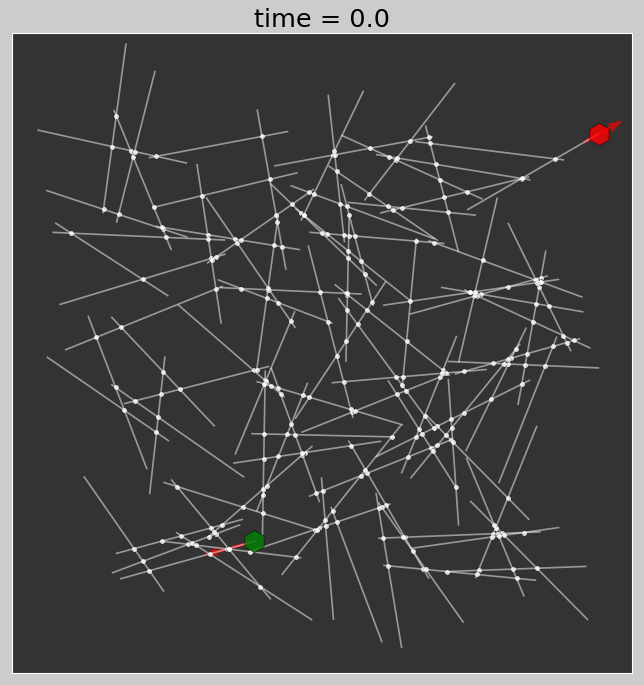
\includegraphics[width=0.7\linewidth]{figure/mpl_plot}
	\caption{}
	\label{fig:mpl_plot}
\end{figure}

\begin{figure}[h]
	\centering
	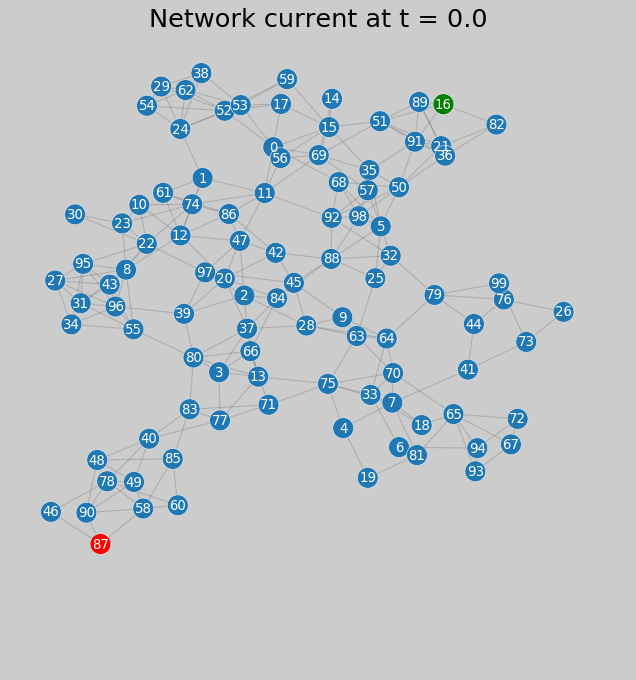
\includegraphics[width=0.8\linewidth]{figure/graph_plot}
	\caption{}
	\label{fig:graph_plot}
\end{figure}

\subsection{\label{sec:level2} Simulation}
When connected to external voltage biases, nanowire networks behave like traditional electrical networks. Each component in the network obeys Kirchhoff's law. Hence the voltage distribution across the network can be obtained by solving \cite{Dorfler2018}:

\begin{equation}
{\cal L}^\dagger V = I,
\end{equation}

where $\mathcal{L}^\dagger$ is the expanded graph Laplacian of the network, composed as:

\begin{equation}
	\cal L^\dagger = 
	\left[
	\begin{array}{c|c}
	\cal L&  C\\ 
	\hline
	C^T & \mathbb{0}  
	\end{array}
	\right],
\end{equation}

in which $\cal L$ is the graph Laplacian and $C$ represents the nodes (wires) connected to external electrodes. 

\begin{equation}
{\cal L} = D - W.
\end{equation}

Here $W$ is the weighted adjacency matrix of the network. The weights on edges are determined based on their conductance:
\begin{equation}
	W_{ij} = A_{ij}G(i,j).
\end{equation}

And $D$ is the weighted degree matrix generated from $W$:
\begin{align}
	d_i = \sum \limits_{k=1}^{N} W_{i,k},\\
	D = \textbf{diag}(d_i).
\end{align}


\subsection{\label{sec:level2} Centrality}
Centrality \textbf{Put some reference here} is an important measure that helps understand the fundamental structures and connectivities of networks. Betweenness centrality of nodes and edges in networks can demonstrate .... Meanwhile, closeness centrality of nodes can be used to interpret the ..... \cite{Newman2010}.

A variation of centrality measures based on current flow model proposed by Brandes and Fleischer \cite{Brandes2005} is employed here. As the electrical dynamics in our networks fall in the class of \textbf{random walks} (not sure about here).

The betweenness centrality of a edge in the networks can be determined by:

\begin{equation}
c_{CB}(e) = \frac{\sum \limits_{s \neq t \in V}\tau_{st}(e)}{(n-1)(n-2)},
\label{eq:ebc}
\end{equation}



where $\tau_{st}(e)$ is the current flow through edge $e$ between nodes $s$ and $t$, while $n$ stands for number of nodes in the network.

The closeness centrality of a node in this context is structured in the same way as normal closeness centrality, with distance measured based on effective resistance rather than graphical distance. Therefore it is given by:

\begin{equation}
	c_{CC}(v) = \frac{n-1}{\sum \limits_{v \neq w \in V} R(v,w)}.
	\label{eq:ecc}
\end{equation}
In the context of a unit $st$-current in the network, $R(v,w)$ represents the effective resistance between nodes $v$ and $w$.

\subsection{\label{sec:level2} Communicability}
Communicability in a network represents .... \cite{Estrada2008}. 

In this work communicability is calculated based on the weighted connections \cite{Crofts2009}. A symmetric matrix $M$ is generated to depict the communicability distribution, where $M_{ij}$ represents the communicability between nodes $i$ and $j$. Therefore, $M$ reads:
\begin{equation}
M = \exp{(D^{-1/2} W D^{-1/2})}.
\end{equation} 

The communicability of a node can be defined as how communicable the node is to the rest of the network, which will have the expression as:

\begin{equation}
	m_i = \sum \limits_{k = 1}^N M_{ik}, \qquad k \neq i.
	\label{eq:ncomm}
\end{equation}



\subsection{\label{sec:level2} Modularity}
Modularity is a network metric that ..... \textbf{talk about it here} \cite{Rubinov2009}.

Recent studies in neuro-science demonstrated that modularity plays an important role in .... \textbf{talk about it here} \cite{Godwin2015}. 
 
Modularity ($Q^w$) in a weighted network can be calculated by the Louvain method \cite{Blondel2008}:
 
% \begin{equation}
% Q^w = \frac{1}{I^w} \sum \limits_{i,j} \left[W_{ij} - \frac{k_i^w k_j^w}{I^w} \right] \delta(m_i, m_j),
% \end{equation}
\begin{equation}
Q^w = \frac{1}{D} \sum \limits_{i,j} \left[W_{ij} - \frac{d_i d_j}{D} \right] \delta(m_i, m_j),
\label{eq:mod}
\end{equation}

in which $w_{i,j}$ is the weight of the edge between nodes $i$ and $j$, $I^w$ represents sum of all weights in the network, $k_i^w$ stands for the weighted degree of node $i$, $m_i$ is the community where node $i$ is located, and $\delta$ is the Kronecker delta function.

\subsection{\label{sec:level2} Transfer Entropy}

Transfer entropy is an effective metric for information transduction ...... \textbf{cite Joe here}.

\begin{equation}
T_{Y \rightarrow X} = \sum \limits_{u_n} p(u_n) \log \frac{p(x_{n+1}| x_n^{(k)}, y_n^{(l)})}{p(x_{n+1}|x_n^{(k)})}.
\end{equation}

$n$ is a time index, $u_n$ represents the state transition tuple $(x_{n+1}, x_n^{(k)}, y_n^{(l)})$, $x_n^{(k)}, y_n^{(l)}$ represent the $k$ and $l$ past values of $x$ and $y$ up to and including time $n$. \textbf{rephrase here}.


The transfer entropy across an edge ($e_{i,j}$) is calculated by:
\textbf{Have to write these equations in a better manner.}

\begin{equation}
TE_{i,j} = T_{V_i \rightarrow V_j}
\end{equation}

And therefore the average outward TE and inward TE of a node can be calculated by:

\begin{equation}
\langle TEout_i \rangle = \frac{\sum \limits_{i,j, A_{i,j} \neq 0} TEout}{\text{\# of edges connected to i}}
\end{equation}

\section{\label{sec:level1} Results }

\subsection{\label{sec:level2} Centrality and Dynamics}

As the network evolves, the edges close to sources and drains will be turned on first. A winner-takes-all current path will be formed, then branches out to the rest of the network. The current paths are more likely to be formed first at the most central positions and then the peripherals. At a specific time $t$, current-flow betweenness centrality of edges can be determined by \ref{eq:ebc}. The edges with higher centrality are more likely to exhibit higher filament state and voltage.

Meanwhile, voltage ($\vec{V_e}$) and filament state ($\vec{\lambda}$) are strongly coupled in the network. Higher voltage on an edge will lead to faster growth of its filament state. In return, higher filament state  means the edge will have a higher conductance (\textbf{refer to equation here}), which increase the chance for the edge to achieve higher voltage.

% Among all sorts of metrics, voltage distribution on nodes $\vec{V_n}$ and on edges $\vec{V_e}$ would be the most interesting ones since the change rate of conductances exhibited by edges are determined by $\vec{V_e}$. Meanwhile changes of conductance at edges will lead to a redistribution of voltage across the voltage.

\paragraph{Filament state}

The absolute values of filament states $|\vec{\lambda (t)}|$ as a function of edge current-flow betweenness centrality are plotted on fig. \ref{fig:v_lam_cent} with its data points colored by corresponding conductance states. The plot shows that edges at more preferable positions will have greater filament growth. The color spectrum on the plot also validates the conductance transition of edges based on their filament states. These high centrality edges are having significantly higher conductance since their filament states are greater than $0.1$, and thus form the first current path.

\paragraph{Voltage distribution} 

Voltage distribution on edges $|\vec{V_e(t)}|$ as a function of centrality is also included in fig. \ref{fig:v_lam_cent} with the same coloring scheme. The data points can be clearly classified into three regimes. The two linear regimes at the left and right ends correspond to the OFF and ON edges. The transition regime in between therefore represents the edges whose conductance are at some middle values in the tunneling model. The plot indicates that within each regime, edges with higher centrality will have higher voltage. The ones who are having higher voltages will be turned on first to form a current path.

\begin{figure}[h]
	\centering
	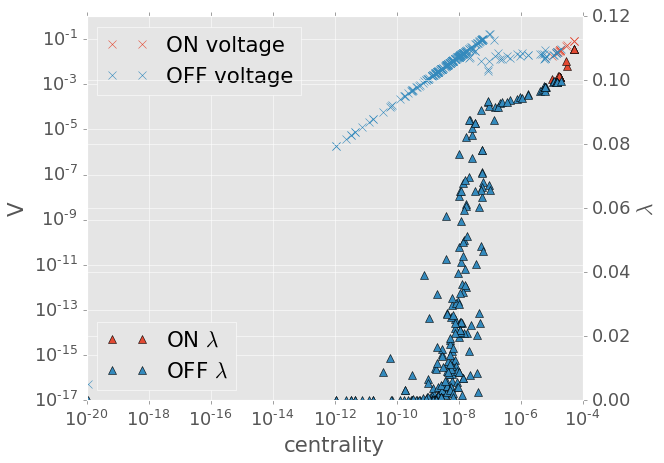
\includegraphics[width=1\linewidth]{figure/v_lam_cent}
	\caption{Absolute values of voltage and filament as a function of centrality at T = 2.9 s. Current path was formed at . Current-flow betweenness centrality is calculated by Eq. \ref{eq:ebc}. The data points are colored based on their corresponding conductance.}
	\label{fig:v_lam_cent}
\end{figure}

\paragraph{Current flow}
\textbf{Not sure if we have  to keep this}
The cumulative current flow through nanowires shows are linear relationship versus node current flow betweenness centrality. fig. \ref{fig:i_cent}.

\begin{figure}[h]
	\centering
	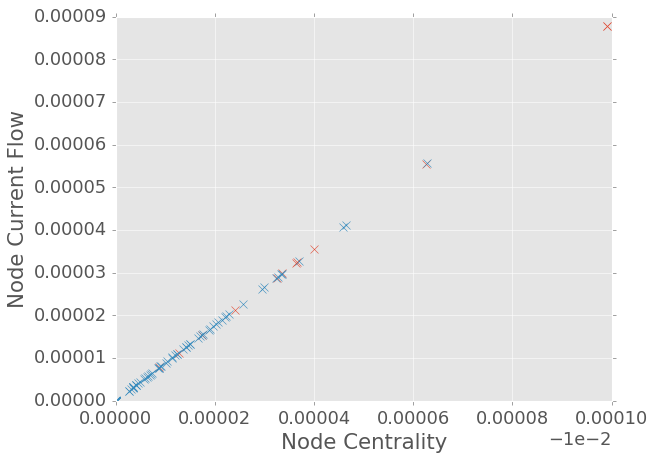
\includegraphics[width=1\linewidth]{figure/I_cent}
	\caption{Current flow on a nanowire vs node centrality}
	\label{fig:i_cent}
\end{figure}

\subsection{\label{sec:level2} Centrality and Functionality}

\textbf{WORDING HERE as well.} Intuitively one would think certain nodes in the network will have a more important role for certain functionalities. Here analysis of the network's functionality such as communicability and transfer entropy are presented.

The communicability of nodes at $t$ can be calculated based on eq. \ref{eq:ncomm}. At an arbitrary time point during the activation (Right after first current path formation here ), when plotted as a function of current-flow closeness centrality on log-log scale, communicability shows as a close to exponential curve, indicating that the nodes at more central positions are more communicable to the rest of the network as this time point. 

% \paragraph{Mean communicability}
% Briefly Introduce the idea of communicability. 

% The communicability matrix ($M$) is generated based on $W$.... Each entry represents .... \textbf{might cite some Comm paper here}.

% The row sum of $M$ can somehow interpret how communicable a node is to the rest of the network.

% The plot of comm vs node closeness cent shows something .....

\begin{figure}[h]
	\centering
	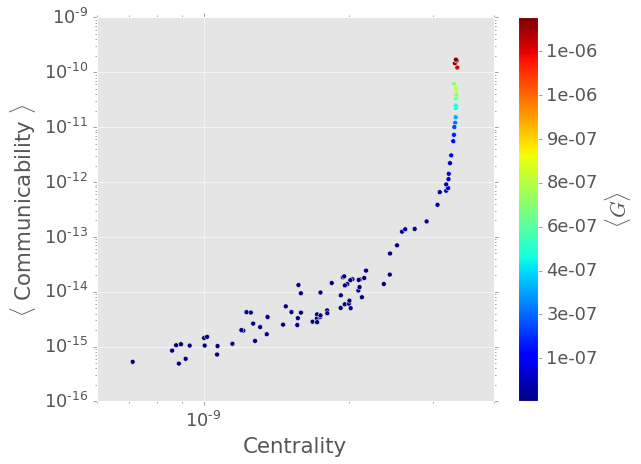
\includegraphics[width=1\linewidth]{figure/comm_cent}
	\caption{\textbf{Node communicability vs closeness centrality at $t = 2 s$.} Node communicability is calculated by eq. \ref{eq:ncomm}. Closeness centrality is calculated by eq. \ref{eq:ecc}. The plot is done on log-log scale. As the nodes at more central positions are having much higher communicabilities (and higher conductance). And the other nodes follows a close to linear trend.}
	\label{fig:comm_cent}
\end{figure}

The node closeness centrality also shows an interesting correlation with transfer entropy. Here in the context of nodes, the in TE and out TE will be the main focus \textbf{Have to write equations to define in and out}. With 50 repetitions of different source/target pairing (while keeping the graphical distance between them constant), TE averaged across the whole time-series shows a close to linear relationship with centrality on semilogy scale. Centrality here is calculated at $t = 0s$, which reflects the structural properties of the network (as all edges are having same weight at $t = 0s$). Nodes at more central positions have the potential to send out and take in more information flows and exhibit richer dynamics.


\begin{figure}[h]
	\centering
	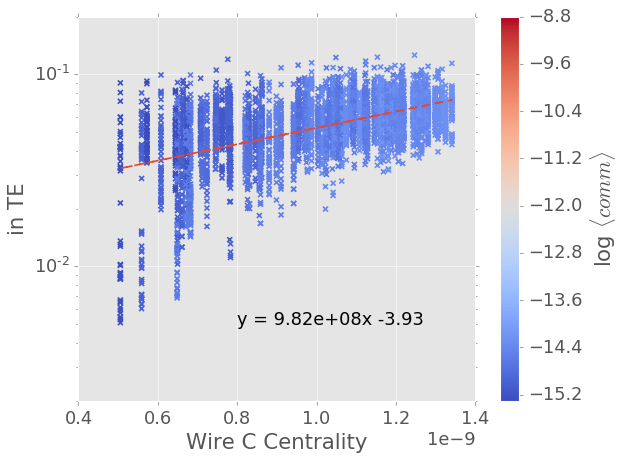
\includegraphics[width=1\linewidth]{figure/in_TE}
	\caption{\textbf{Might not need color here. Node in TE as a function of centrality. (Out TE in  supplement)} TE is calculated based on Eq \textbf{equation}. Node centrality is calculated based on the current-flow closeness algorithm at $t = 0$. Communicability is calculated by Eq \textbf{equation} at $t = 0$ as well. 50 simulations with different source-drain pairings are done on the same 100 network. All the source-drain pairings are controlled to have same graphical distance. Identical Mackey-Glass signals are applied to these simulations to activate the network. Each data point on the plot represent one node in one simulation. A close to linear correlation between TE and centrality can be determined from the plot, which means nodes with higher centralities tend to have richer dynamics for taking in and sending out information.}
	\label{fig:in_te}
\end{figure}

Fig. \ref{fig:TE_cent_act} shows the in TE vs C centrality around the time when the first current path forms. On a semilogy scale, the high centrality nodes (centrality calculated at $T = 1.5 s$) are having similar TE and high communicabilities. These are mainly the nodes connected to the ON edges. The low centrality nodes on the other hand indicates that with higher centralities there will be higher TE, which is consistent with our analysis in fig. \ref{in_te}.

\begin{figure}[h]
	\centering
	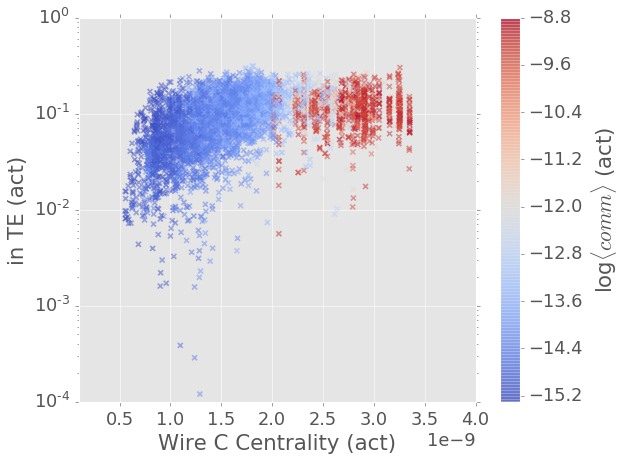
\includegraphics[width=1\linewidth]{figure/TE_cent_act}
	\caption{\textbf{inTE vs closeness centrality around activation.} The same activation test is done as fig. \ref{fig:in_te}.	TE is averaged in a $0.2s$ window right before the activation (mainly to cancel out the randomness). Centrality is measured at the current path formation time. The high centrality nodes are the ones connected to ON edges. They exhibit high communicabilities and high in/out TEs. The nodes in the low centrality group on the other hand indicates that with higher centrality, the nodes will have higher in/out TEs, and thus more capable for information transfer.}
	\label{fig:TE_cent_act}
\end{figure}


% \paragraph{Node Active Information Storage}
% \textbf{Not sure whether we need it here}.

\subsection{Time-series analysis}

\begin{figure}
	\centering
	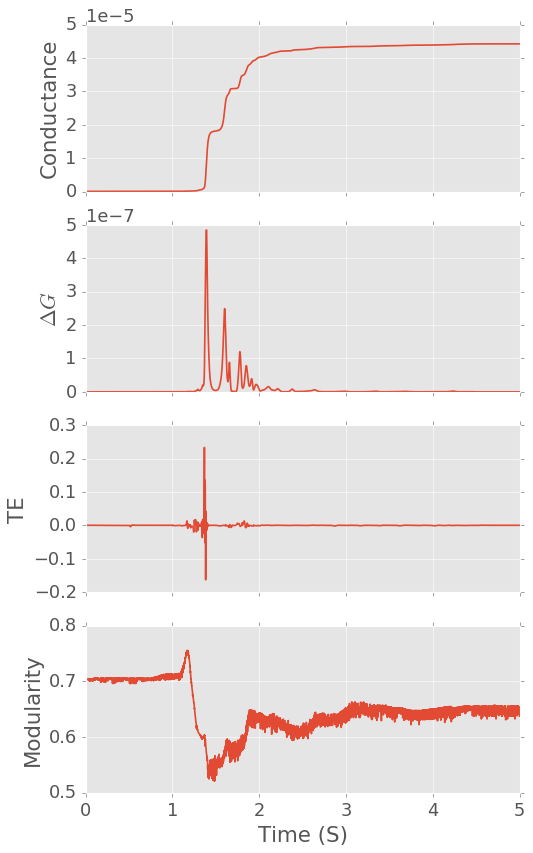
\includegraphics[width=1\linewidth]{figure/time_series}
	\caption{\textbf{Time series data for network measures.} The dashed vertical green line represents the 			time of first current path formation.
			\newline (a) Collective conductance of network as a function of time. The collective conductance started increasing when the first edge is turned on. The growth will slow down after the first current path is formed.
			\newline (b) The time derivative of conductance. The derivative is calculated using second order accurate central differences on the collective conductance time series data. The growth regime of conductance shows a great correspondence of $\Delta G$'s spikes.
			\newline (c) Transfer entropy as a function of time. The transfer entropy time series data here is calculated with the Kraskov estimator and averaged across the network. A moving average with window size of 100 is applied to smooth the curve. Transfer entropy in the activation period is significantly higher than the rest.
			\newline (d) Modularity as a function of time. The weighted modularity of network is calculated by Louvain method(Eq. \ref{eq:mod}) As the network evolves, modularity will first increase as high conductance edges are spread across the network and having their own communities. With the formation of the first current path, the modularity will have a significant drop since these isolating communities are connected. Then the modularity will keep having such fluctuations with smaller scales as more edges are turned on and forming new current paths.}
	\label{fig:time_series}
\end{figure}

Time series analysis of the network's activation can be even more intriguing. As plotted in Fig. \ref{fig:time_series}(a), the activation of the network mainly have three regimes - the resting (\textbf{maybe another word} ?ground ?low-conductance) regime, the transition regime and the stable (?equilibrium ?high-conductance) regime. Key events of the activation also coincide with each other on time scale. 


In the resting regime, the junctions are all OFF. Collective conductance of the network remains low. Filament states on junctions start to grow based on their voltage. Increase of conductance will first take place at junctions with preferred positions. Information flow is high when the signal first came in, but in general at a low level in this regime. The modularity level stays constant when all junctions are at low-conductance state. A peak in modularity will then emerge when certain junctions in the network starts to have higher conductances as they are forming "highlands". When more junctions experience conductance increase, modularity starts to drop.

The transition regime starts when the first switches are turned on (\textbf{Here it's the tunneling model so maybe some other wording. Like some switches are exhibiting higher conductance}). Collective conductance of the network starts to increase significantly as the time derivative will have a spike. Modularity of the network reaches the bottom level \textbf{wording here}. With more junctions turned ON, the first current path (winner-takes-all) will be formed and the conductance keeps increasing with a lower path. Modularity starts to increase again as the nodes on the current path stands out from the rest of the network. Information flow will increase to a higher scale (A spike in Gaussian data). 

The transition regime ends when most junctions are at high-conductance states (the rest are not reachable with this specific source-drain pairing). Collective conductance will be stable at a high level. Information flow will decrease to a lower scale similar to the resting regime. The modularity will also be stable in this regime.

Snapshots of the network in different phases shown in fig. \ref{fig:network_comparison}. Nodes are colored with the sum of inTE and outTE averaged in the last $0.2 s$ time window. Similarly, edges are colored by the sum of the TE flows in both direction in the last $0.2$ time window. (Kraskov estimator is used here.) At $t= 0.5$, the whole network is at rest. None of the nodes or edges are having significant information transfer. When the first current path is formed at $t = 1.465 s$, some nodes and edges start to have significant information flow, but most flows are happening around the central nodes. When $t = 2.0 s$, the information flow is even stronger as more nodes are having high in and out TEs. Meanwhile, even nodes at peripheral positions are having significant information flow. After the network is in the equilibrium regime for a while ($t = 2.5s$), the information flows decay as the local TE values are significantly lower than the transition regime.

\begin{figure*}[h]
	\centering
	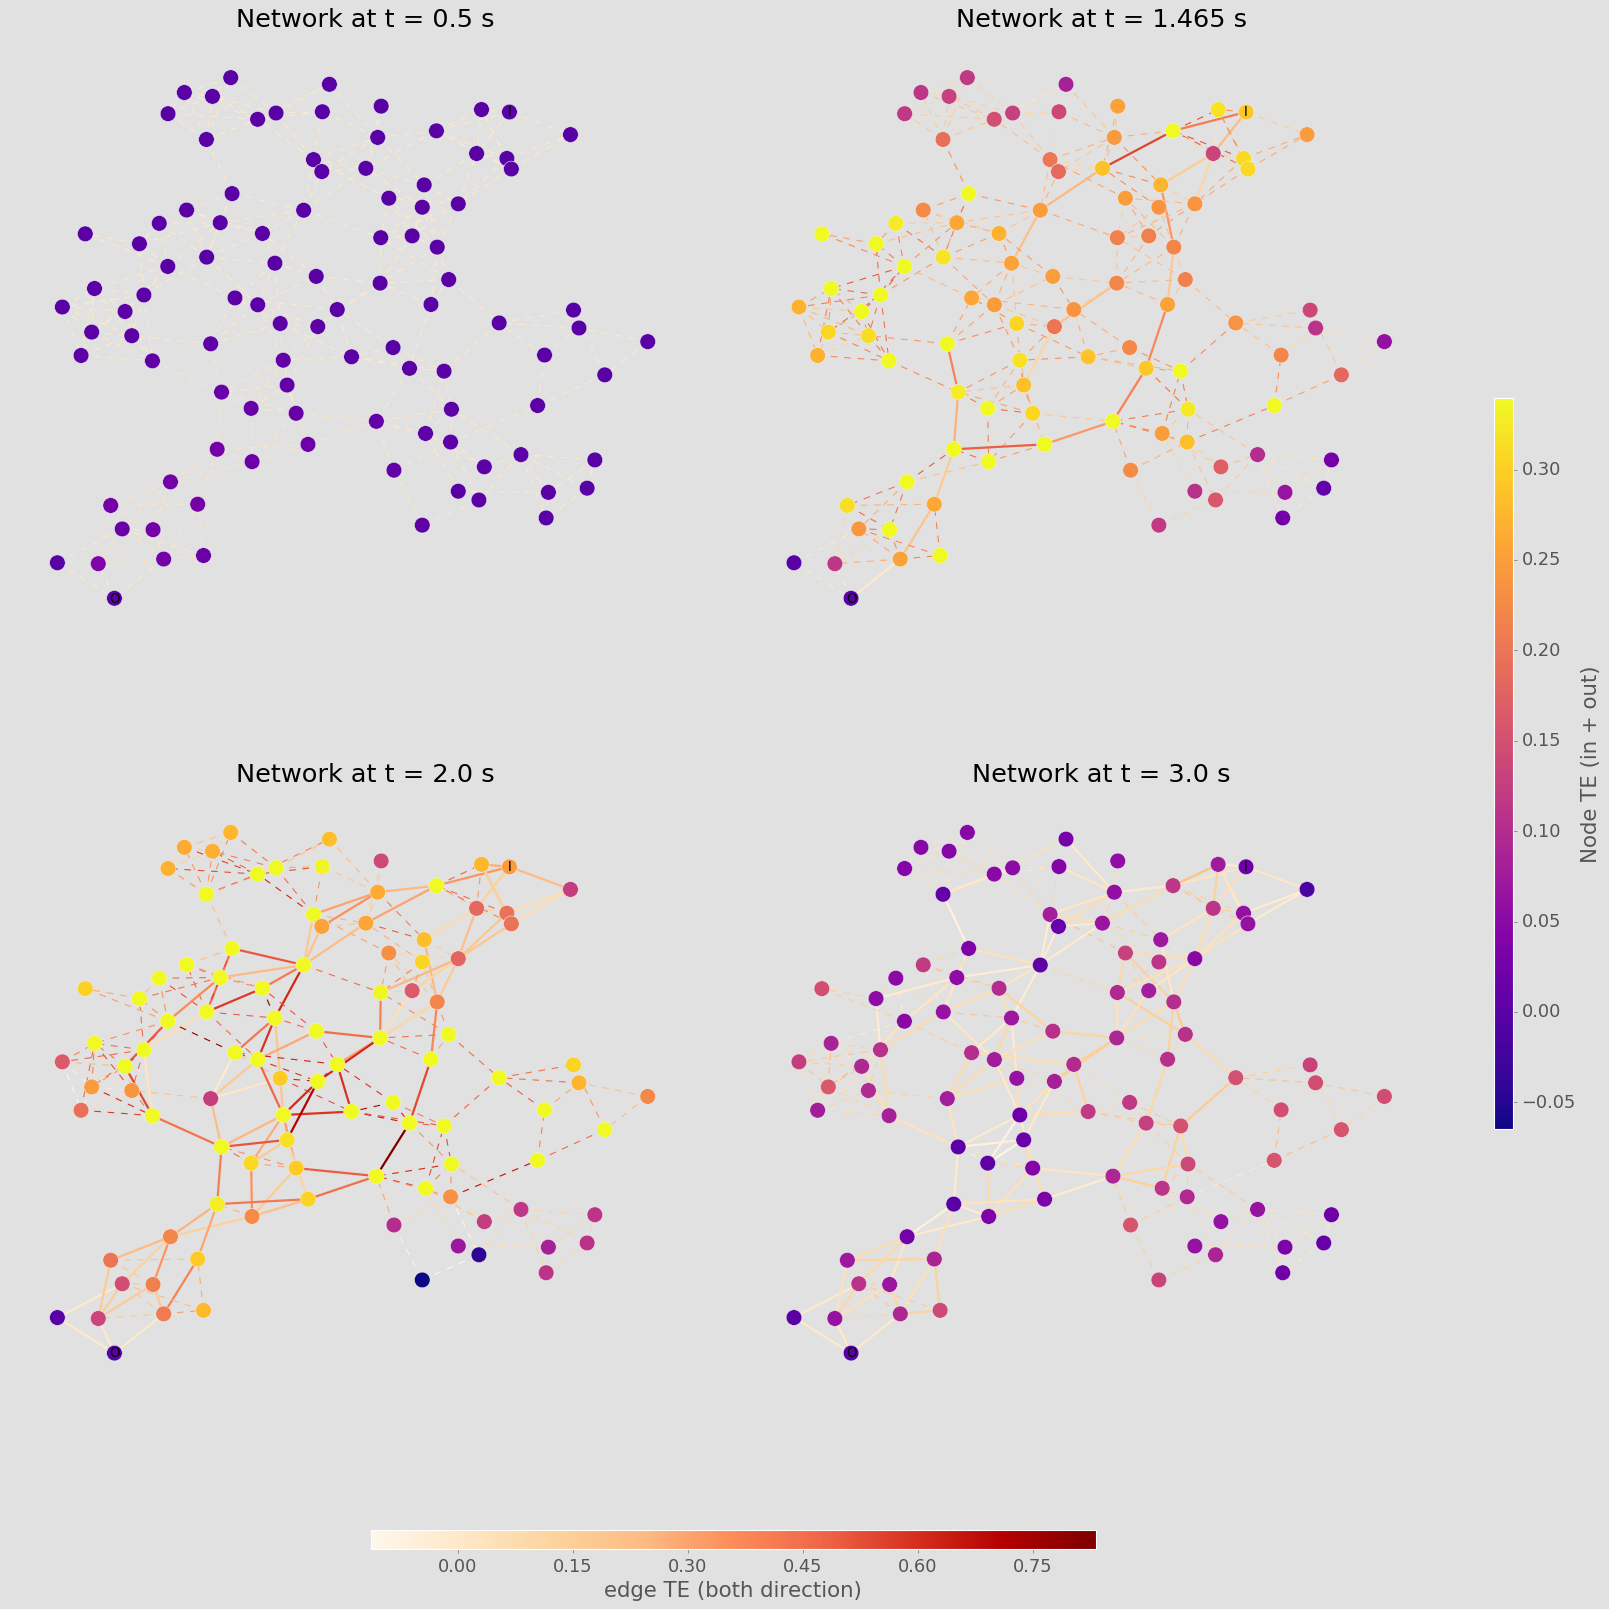
\includegraphics[width = 0.8\paperwidth]{figure/time_network_comparison}
	\caption{\textbf{Network information flow snapshots at different time points.}
			Snapshots of the network are taken at time points before activation ($t = 0.5s$), when the first current path formation ($t=1.465s$), when the network finishes large scale activation ($t = 2s$) and when the network is stable with high collective conductance ($t = 2.5s$).
			Nodes are colored with time-averaged TE flow (inTE + outTE) within the last 0.2 second window using the Kraskov estimator. Edges are colored by the sum of corresponding transfer entropy in both directions. TEs are increasing when the network is being activated and richer dynamics emerge. After the network reaches a stable state (t = 2.5 s), the TEs activities decay as well.}
	\label{fig:network_comparison}
\end{figure*}

A more thorough validation of the hypothesis is done activating the same network with different source-drain pairings. The graphical distance between source and drain in each repetition is controlled to be constant. Identical Mackey-Glass signals with arbitrary amplitude (\textbf{maybe another word like strength/ xxx parameter}) between $2-5 V$ are delivered to the network. The times when the key events take place are recorded and plotted as fig. \ref{fig:time_align}. \textbf{Wording HERE} With the current path formation time on the x-axis, times for other key events line up fairly well. When the amplitude is larger, the first current path will be formed earlier and similar for other events. With amplitude ? greater than 3.5V, the key events line up linearly. With small amplitudes, the activation takes more time and thus more fluctuations in the dynamics are captured. These fluctuations contributes to the outliers in the plot.


% \paragraph{$\Delta G$}

% The conductance time-series of the network reflects the activation stage of the network. Specifically, $\Delta G$ can help identify the avalanche behaviors of the network.


% \paragraph{TE time series}

% The transfer entropy across the whole network is calculated in the same way as before. The average is taken over the whole network the time series to obtain the time series.

% Plotting TE time-series together with $\Delta G$ in the same figure, the spikes of both curves coincide.

% Different amplitude of voltage biases are applied to the network. The activation time and TE peak time in these realizations line-up pretty well.

% \paragraph{Modularity time series}

% Modularity of the network is calculated throughout the activation. The drop of Modularity coincide with $\Delta G$ as well. 

\begin{figure}[h]
	\centering
	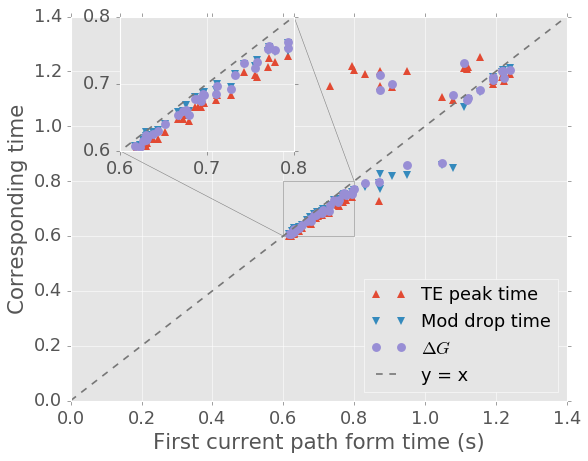
\includegraphics[width=1\linewidth]{figure/time_align}
	\caption{\textbf{Key events time as functions of first current path formation time.} 
			The same 100 network is used for 50 simulations with different source-drain pairings. The graphical distances between sources and drains are controlled to be constant. Identical Mackey-Glass signal with random amplitudes ranging between 2-5 V are applied to these simulations. Simulations with higher amplitudes will form current paths earlier. 
			\newline 
			X-axis represents the current path formation time in different simulations. Y-axis represents the corresponding time for key events to take place in these simulations. As shown in this figure, key events such as $\Delta G$ maximum, TE spike (in Gaussian estimation) and modularity drop will happen around the first current path formation time. 
			\newline
			\textbf{Rephrase here} Thus the network will be optimal for information processing and specific task around the transition phase when the first current path is forming and the network is turning on. }
	\label{fig:time_align}
\end{figure}






\newpage
\subsection{Pre activation task}


Pre-activate the network with Mackey-Glass signal, extract the state from different time-points. Then do a non-linear signal transform on it. 

Hypothesis: a network at certain modularity level (or initial modularity level) might do a better job in tasks.

A 100 network is activated with Mackey-Glass signal. It's modularity time-series is shown in \ref{fig:pre_act_task}. As discussed in the result section, the modularity level of the network can somehow reflect the network's current state. Then the network's corresponding state (conductance and filament state) at times between $t = 0 - 2 s$ are extracted. Non-linear transformation task is then applied to the network starting from those extracted states. \textbf{x-axis in plot should be changed.}

Fig. \ref{fig:pre_act_task}(b) shows that ...

A t-test is done ....


\begin{figure}[h]
	\centering
	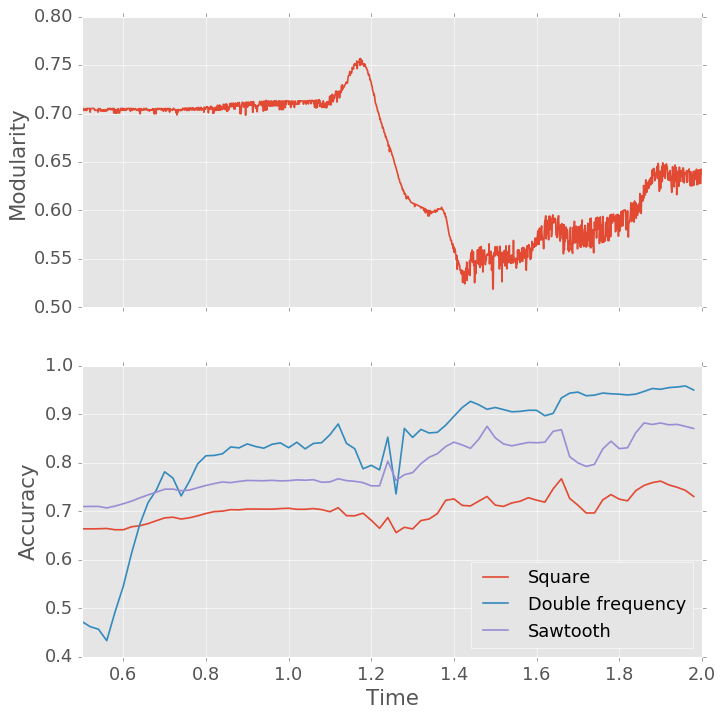
\includegraphics[width=1\linewidth]{figure/pre_act_task}
	\caption{}
	\label{fig:pre_act_task}
\end{figure}

% The Guimera \textbf{cite here} plots can be displayed as follow:
 
% \begin{figure}[h]
% 	\centering
% 	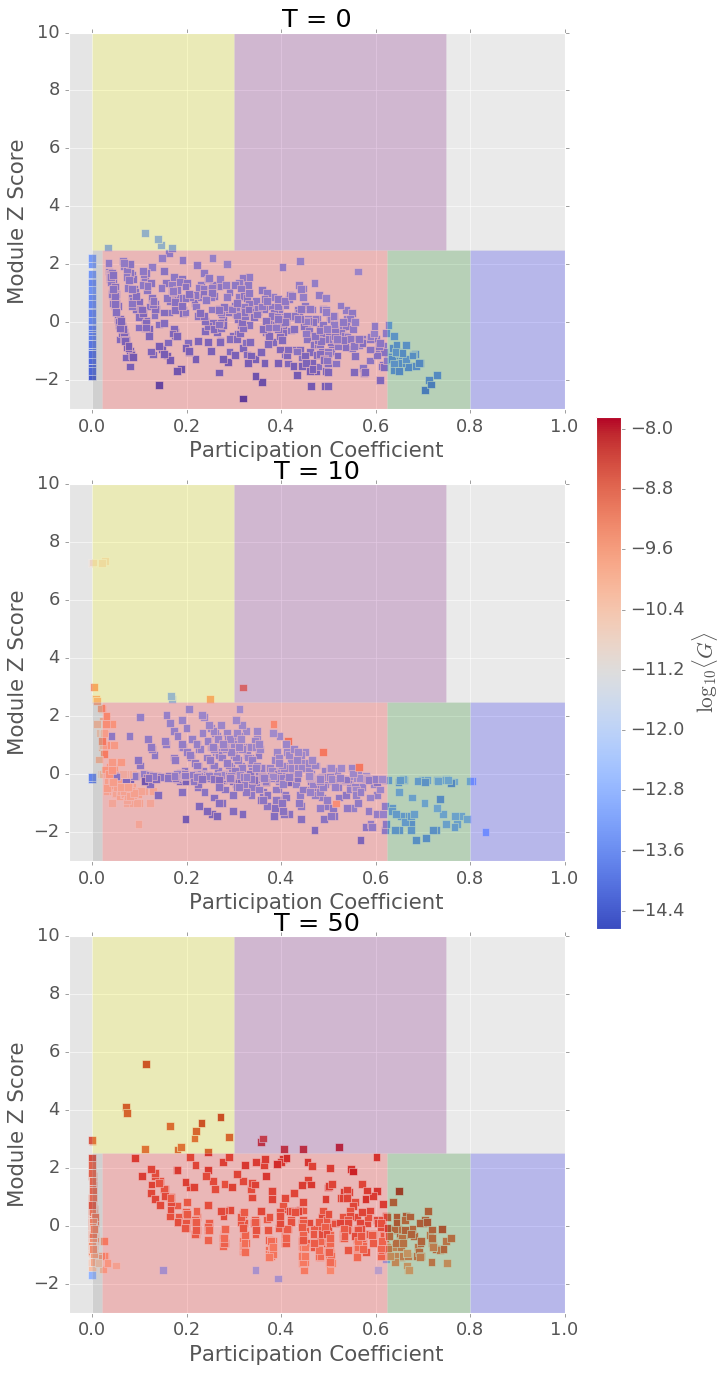
\includegraphics[width=1\linewidth]{figure/guimera_combine}
% 	\caption{}
% 	\label{fig:guimera_combine}
% \end{figure}

% \textbf{Have to match the color bars here.}

\newpage
\section{\label{sec:level1} Discussion}

\section{\label{sec:level1} Conclusion}








\begin{acknowledgments}
We wish to acknowledge the support of the author community in using
REV\TeX{}, offering suggestions and encouragement, testing new versions,
\dots.
\end{acknowledgments}

\appendix

\section{Appendixes}



\section{A little more on appendixes}



% The \nocite command causes all entries in a bibliography to be printed out
% whether or not they are actually referenced in the text. This is appropriate
% for the sample file to show the different styles of references, but authors
% most likely will not want to use it.
\nocite{*}



\bibliography{paper1} \label{paper1}% Produces the bibliography via BibTeX.

\end{document}
%
% ****** End of file apssamp.tex ******
